\section{Software}
\begin{frame}{Software}
	Our project is \stress{openly} and \stress{actively} developed on
	\vcenteredinclude{
\includegraphics[height=2ex]{figures/software_logos/octocat.pdf}\hspace{-0.05cm}
	
\includegraphics[height=2ex]{figures/software_logos/github.pdf}}\\
	{\color{purple}\url{https://github.com/RD-clustering/B_decays_clustering}}
	
	\bigskip
	Implemented in \vcenteredinclude{
\includegraphics[height=3ex]{figures/software_logos/python.pdf}} using
	\begin{itemize}
		\item \vcenteredinclude{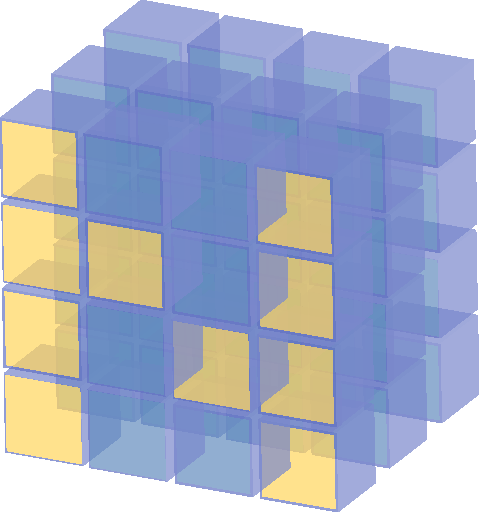
\includegraphics[height=4ex]{figures/software_logos/numpy_noname.pdf}} \texttt{numpy} {\footnotesize(fast numeric operations on arrays)}
		\item \vcenteredinclude{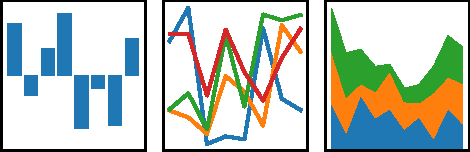
\includegraphics[height=3.5ex]{figures/software_logos/pandas_noname.pdf}} \texttt{pandas} {\footnotesize(dataframes)}
		\item \vcenteredinclude{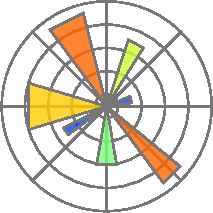
\includegraphics[height=4ex]{figures/software_logos/matplotlib.pdf}} \texttt{matplotlib} {\footnotesize(beautiful plots)}
		\item \vcenteredinclude{
\includegraphics[height=3.5ex]{figures/software_logos/sklearn.pdf}} \texttt{scikit-learn} {\footnotesize(clustering tools)}
		\item \vcenteredinclude{
\includegraphics[height=3.5ex]{figures/software_logos/scipy.pdf}} \texttt{scipy} {\footnotesize(integration and clustering tools)}
		\item \vcenteredinclude{
\includegraphics[height=3.5ex]{figures/software_logos/jupyter.pdf}} \texttt{jupyter} {\footnotesize(interactive notebooks)}
		\item \vcenteredinclude{
\includegraphics[height=3ex]{figures/software_logos/wcxf.pdf}} \texttt{wcxf} {\footnotesize(specify Wilson coefficients in a variety of bases)}
		\item \vcenteredinclude{
\includegraphics[height=3ex]{figures/software_logos/wilson.pdf}} \texttt{Wilson} {\footnotesize(running of Wilson coefficients)}
		\item \vcenteredinclude{
\includegraphics[height=3ex]{figures/software_logos/flavio.pdf}} \texttt{Flavio} {\footnotesize(various observables with NP predictions)}
	\end{itemize}
\end{frame}


\begin{frame}{Software}
	General steps:
	\begin{enumerate}
		\item \stress{Scan}: Calculate binned distributions for your observable, e.g. $\dd\Gamma/\dd q^2$
		\begin{itemize}
			\item An arbitrary python function can be specified
			\item E.g. simply take an observable from \texttt{flavio}
			\item Parallel processing supported
		\end{itemize}
		\item (optional) \stress{Add errors}: Easy interface to add various kinds of errors {\footnotesize(Poisson, flat relative errors, errors given by covariance matrix, maximally correlated errors etc.)}
		\item \stress{Cluster}: Take the binned distributions and cluster them\\
		{\footnotesize Clustering class is subclassed to support any clustering algorithm}
		\item \stress{Plot}: Various plotting methods are provided
	\end{enumerate}
\end{frame}

\begin{frame}{Software}{Quick tutorial}
	Generate a sample of kinematic distributions (here $\dd\Gamma/\dd q^2$ for $\bdstaunu$) using the {\ttfamily\hlkwd{Scanner}} class:\\[2ex]
	
	{
		\noindent
		\ttfamily\small
		\hlstd{s\ }\hlopt{=\ }\hlstd{}\hlkwd{Scanner}\hlstd{}\hlopt{()}\hspace*{\fill}\\
		\hlstd{s}\hlopt{.}\hlstd{}\hlkwd{set\textunderscore dfunction}\hlstd{}\hlopt{(}\hspace*{\fill}\\
		\hlstd{}\hlstd{\ \ \ \ }\hlstd{bdlnu}\hlopt{.}\hlstd{dGq2}\hlopt{,}\hspace*{\fill}\\
		\hlstd{}\hlstd{\ \ \ \ }\hlstd{binning}\hlopt{=}\hlstd{np}\hlopt{.}\hlstd{}\hlkwd{linspace}\hlstd{}\hlopt{(}\hlstd{bdlnu}\hlopt{.}\hlstd{q2min}\hlopt{,\ }\hlstd{bdlnu}\hlopt{.}\hlstd{q2max}\hlopt{,\ }\hlstd{}\hlnum{10}\hlstd{}\hlopt{),}\hspace*{\fill}\\
		\hlstd{}\hlstd{\ \ \ \ }\hlstd{normalize}\hlopt{=}\hlstd{}\hlkwa{True}\hspace*{\fill}\\
		\hlstd{}\hlopt{)}\hspace*{\fill}\\
		\hlstd{s}\hlopt{.}\hlstd{}\hlkwd{set\textunderscore wpoints\textunderscore equidist}\hlstd{}\hlopt{(}\hspace*{\fill}\\
		\hlstd{}\hlstd{\ \ \ \ }\hlstd{}\hlopt{\{}\hspace*{\fill}\\
		\hlstd{}\hlstd{\ \ \ \ \ \ \ \ }\hlstd{}\hlstr{"CVL\textunderscore bctaunutau"}\hlstd{}\hlopt{:\ ({-}}\hlstd{}\hlnum{0.3}\hlstd{}\hlopt{,\ }\hlstd{}\hlnum{0.3}\hlstd{}\hlopt{,\ }\hlstd{}\hlnum{10}\hlstd{}\hlopt{),}\hspace*{\fill}\\
		\hlstd{}\hlstd{\ \ \ \ \ \ \ \ }\hlstd{}\hlstr{"CSL\textunderscore bctaunutau"}\hlstd{}\hlopt{:\ ({-}}\hlstd{}\hlnum{0.3}\hlstd{}\hlopt{,\ }\hlstd{}\hlnum{0.3}\hlstd{}\hlopt{,\ }\hlstd{}\hlnum{10}\hlstd{}\hlopt{),}\hspace*{\fill}\\
		\hlstd{}\hlstd{\ \ \ \ \ \ \ \ }\hlstd{}\hlstr{"CT\textunderscore bctaunutau"}\hlstd{}\hlopt{:\ ({-}}\hlstd{}\hlnum{0.4}\hlstd{}\hlopt{,\ }\hlstd{}\hlnum{0.4}\hlstd{}\hlopt{,\ }\hlstd{}\hlnum{10}\hlstd{}\hlopt{)}\hspace*{\fill}\\
		\hlstd{}\hlstd{\ \ \ \ }\hlstd{}\hlopt{\},}\hspace*{\fill}\\
		\hlstd{}\hlstd{\ \ \ \ }\hlstd{scale}\hlopt{=}\hlstd{}\hlnum{5}\hlstd{}\hlopt{,}\hspace*{\fill}\\
		\hlstd{}\hlstd{\ \ \ \ }\hlstd{eft}\hlopt{=}\hlstd{}\hlstr{'WET'}\hlstd{}\hlopt{,}\hspace*{\fill}\\
		\hlstd{}\hlstd{\ \ \ \ }\hlstd{basis}\hlopt{=}\hlstd{}\hlstr{'flavio'}\hlstd{}\hspace*{\fill}\\
		\hlopt{)}\hspace*{\fill}\\
		\hlstd{s}\hlopt{.}\hlstd{}\hlkwd{run}\hlstd{}\hlopt{()}\hspace*{\fill}
		\hlstd{\hspace*{\fill}\\
			s}\hlopt{.}\hlstd{}\hlkwd{write}\hlstd{}\hlopt{(}\hlstd{}\hlstr{"output/scan"}\hlstd{}\hlopt{,\ }\hlstd{}\hlstr{"tutorial"}\hlstd{}\hlopt{)}\hlstd{}\hspace*{\fill}\\
		\mbox{}
		\normalfont
		\normalsize
	}
\end{frame}


\begin{frame}{Software}{Quick tutorial}
	Now we cluster it: \\[2ex]
	
	{
		\noindent
		\ttfamily
		\hlstd{c\ }\hlopt{=\ }\hlstd{}\hlkwd{HierarchyCluster}\hlstd{}\hlopt{(}\hlstd{}\hlstr{"output/scan"}\hlstd{}\hlopt{,\ }\hlstd{}\hlstr{"tutorial"}\hlstd{}\hlopt{)}\hspace*{\fill}\\
		\hlstd{c}\hlopt{.}\hlstd{}\hlkwd{build\textunderscore hierarchy}\hlstd{}\hlopt{()}\hspace*{\fill}\\
		\hlstd{c}\hlopt{.}\hlstd{}\hlkwd{cluster}\hlstd{}\hlopt{(}\hlstd{max\textunderscore d}\hlopt{=}\hlstd{}\hlnum{0.1}\hlstd{}\hlopt{)}\hspace*{\fill}\\
		\hlstd{}\hspace*{\fill}\\
		\hspace*{\fill}\\
		\mbox{}
		\normalfont
		\normalsize
	}
	
	And can have fun plotting: \\[2ex]
\end{frame}